\documentclass[conference]{IEEEtran}
\IEEEoverridecommandlockouts
% The preceding line is only needed to identify funding in the first footnote. If that is unneeded, please comment it out.
%Template version as of 6/27/2024

\usepackage{cite}
\usepackage{amsmath,amssymb,amsfonts}
\usepackage{algorithmic}
\usepackage{graphicx}
\usepackage{textcomp}
\usepackage{xcolor}
\makeatletter
\setlength{\@dblfptop}{0pt}
\setlength{\@dblfpbot}{0pt plus 1fil}
\makeatother
\setlength{\textfloatsep}{8pt plus 2pt minus 2pt}
\setlength{\floatsep}{6pt plus 2pt minus 2pt}
\setlength{\intextsep}{6pt plus 2pt minus 2pt}
\def\BibTeX{{\rm B\kern-.05em{\sc i\kern-.025em b}\kern-.08em
    T\kern-.1667em\lower.7ex\hbox{E}\kern-.125emX}}
\begin{document}

\title{Detekcia zmien prostredia pri komunitných čistiacich akciách}
\author{\IEEEauthorblockN{Oleksii Haiduk}
\IEEEauthorblockA{\textit{FEI} \\
\textit{Technická univerzita v Košiciach}\\
Košice, Slovensko}
\and
\IEEEauthorblockN{Maksym Streltsov}
\IEEEauthorblockA{\textit{FEI} \\
\textit{Technická univerzita v Košiciach}\\
Košice, Slovensko}
}
\maketitle

\begin{abstract}
Táto práca sa zaoberá detekciou zmien medzi dvojicami fotografií zachytávajúcich to isté miesto pred a po komunitnej čistiacej akcii. Cieľom je lokalizovať oblasti, z ktorých bol odstránený odpad, a zároveň odhadnúť rozsah vyzbieraného materiálu pomocou plochy zmeny, počtu objektov alebo jednoduchého skóre vyčistenia. Navrhovaný systém zahŕňa zarovnanie snímok, kompenzáciu rozdielov v osvetlení a perspektíve a následnú detekciu zmien pomocou klasických aj hlbokých metód. V projekte porovnávame viacero implementovaných prístupov, konkrétne klasickú diferenciáciu obrazu po zarovnaní pomocou SIFT + RANSAC, model ChangeFormer, reprezentácie DINOv2, klasifikátor EfficientNet, Siamese U-Net a segmentačný prístup YOLOv8-seg. Výkonnosť systému budeme hodnotiť pomocou metrík ako IoU, Dice a chyby pri odhade množstva odpadu, pričom sledujeme aj odolnosť voči zmenám uhla záberu, prítomnosti ľudí a sezónnym či svetelným podmienkam.
\end{abstract}

\begin{IEEEkeywords}
detekcia zmien, komunitné čistiace akcie, odpad, image registration, change detection, segmentácia
\end{IEEEkeywords}

\section{Úvod a motivácia}
Komunitné čistiace akcie vytvárajú prirodzený scenár pre analýzu zmien prostredia: na rovnakom mieste vznikne dvojica záberov pred zásahom a po ňom. Takéto snímky obsahujú informáciu nielen o tom, že sa odpad odstránil, ale aj o tom, kde sa nachádzal, akú plochu zaberal a ako výrazne sa zmenila vizuálna štruktúra scény. Z pohľadu praktického využitia je to dôležité pri dokumentovaní výsledkov dobrovoľníckych aktivít, pri plánovaní ďalších zásahov aj pri spätnom vyhodnocovaní efektivity čistenia.

Hlavným problémom je, že pred a po fotografie sú v reálnych podmienkach často nezarovnané. Líšia sa uhlom snímania, vzdialenosťou od scény, osvetlením, prítomnosťou ľudí aj sezónnymi zmenami pozadia. Preto nestačí jednoduché porovnanie pixelov bez predspracovania. V projekte sa preto sústreďujeme na pipeline, ktorá najprv fotografie zarovná a až potom hľadá zmeny pomocou klasických aj hlbokých metód.

Naša implementácia zahŕňa viacero prístupov, aby bolo možné porovnať ich správanie v rovnakom vstupnom scenári. Klasická vetva používa SIFT + RANSAC a diferenčný obraz v prekrytej oblasti \cite{lowe2004distinctive,fischler1981random}. Hlbšie prístupy zastupuje ChangeFormer \cite{changeformer2021}, ktorý sa pri nedostupnosti knižníc automaticky prepína do klasického CV fallbacku, ďalej DINOv2 na vizuálne reprezentácie \cite{oquab2023dinov2}, EfficientNet pre odhad čistého a znečisteného stavu \cite{tan2019efficientnet}, Siamese U-Net pre párové spracovanie snímok \cite{daudt2018fully} a YOLOv8-seg pre segmentáciu odpadu \cite{ultralyticsyolo}. Cieľom nie je iba označiť zmenu, ale aj čo najpresnejšie lokalizovať odstránený odpad a získať aspoň približný odhad rozsahu vyzbieraného materiálu.

V ďalších častiach práce budeme porovnávať tieto prístupy na rovnakých dvojiciach snímok a vyhodnocovať ich pomocou metrík ako IoU, Dice, prípadne chyby pri odhade množstva odpadu. Zároveň nás zaujíma robustnosť voči skutočným podmienkam, v ktorých sa komunitné akcie odohrávajú, teda voči meniacemu sa uhlu pohľadu, osvetleniu a rušivým objektom v scéne.

Ako spoločný príklad vstupnej dvojice pre všetky metódy používame dvojicu fotografií uvedenú na obrázku \ref{fig:sample_pair}. Ide o referenčné snímky pred a po vyčistení, ktoré slúžia na ukážku práce jednotlivých algoritmov v jednom porovnateľnom scenári.

\begin{figure}[htbp]
\centering
\begin{minipage}[t]{0.48\columnwidth}
\centering
\includegraphics[width=\linewidth,angle=270]{\detokenize{foto/vzorec do.JPG}}
\caption*{(a) Pred vyčistením}
\end{minipage}
\hfill
\begin{minipage}[t]{0.48\columnwidth}
\centering
\includegraphics[width=\linewidth,angle=270]{\detokenize{foto/vzorec po.JPG}}
\caption*{(b) Po vyčistení}
\end{minipage}
\caption{Ilustračná dvojica fotografií použitá ako spoločný vstupný príklad pre všetky metódy.}
\label{fig:sample_pair}
\end{figure}

\section{Datová sada}
Priamy dataset párov pred a po vyčistení vybraného miesta momentálne neexistuje, preto bolo potrebné vytvoriť vlastný dátový súbor manuálne.

Náš dataset v priečinku \textit{Garbage Pairs Dataset} obsahuje 49 párových zložiek, ktoré obsahujú použiteľnú dvojicu snímok pred a po vyčistení. 
V rámci datasetu sa nachádzajú tri typy párov: páry pochádzajúce z internetu, páry nasnímané vlastnou činnosťou a páry, pri ktorých bola fotografia od odpadu vyčistená pomocou AI.
Pre 14 párov fotografií sme vytvorili aj vlastné binárne masky odstráneného odpadu. Tieto masky sú uložené v priečinku \textit{!masks\_for\_training} a slúžia najmä na tréning a vyhodnotenie segmentačných a change-detection modelov. Masky označujú oblasti, kde sa po vyčistení zmenila scéna a odpad bol odstránený.

\section{Programová pipeline a funkčnosť}
Naše riešenie je grafická aplikácia. Používateľ si vyberie priečinok s dvojicou fotografií, zvolí metódu a spustí spracovanie. Nastavenie jednotlivých modelov prebehne automaticky podľa zvolenej metódy. Po výbere vstupného priečinka program automaticky identifikuje dvojicu snímok pred a po vyčistení podľa názvov súborov a následne spustí vybraný model v príslušnom conda prostredí. Tento postup je dôležitý preto, aby každá metóda fungovala izolovane so svojimi vlastnými závislosťami a neovplyvňovala ostatné modely.

Samotný spracovací tok má rovnaký základ pre všetky metódy. Najprv sa načítajú vstupné snímky, potom sa vykoná zarovnanie dvojice, aby sa znížil vplyv rozdielneho uhla snímania a posunu kamery. Následne sa podľa zvolenej metódy vytvorí mapa zmeny, segmentačná maska alebo skóre vyčistenia. Výsledok sa uloží vo forme textového súhrnu, metrík a vizuálnych artefaktov, ako sú overlay snímky, heatmapa alebo výsledný preview panel.

Používateľské rozhranie zobrazuje vstupnú dvojicu, výsledný panel a textový blok s metrikami a diagnostikou. Po spracovaní sa priečinok s uloženými výsledkami otvorí automaticky. Obrázok \ref{fig:interface} ukazuje hlavné okno aplikácie s výberom priečinka, voľbou metódy a panelom výsledkov.

\begin{figure}[htbp]
\centerline{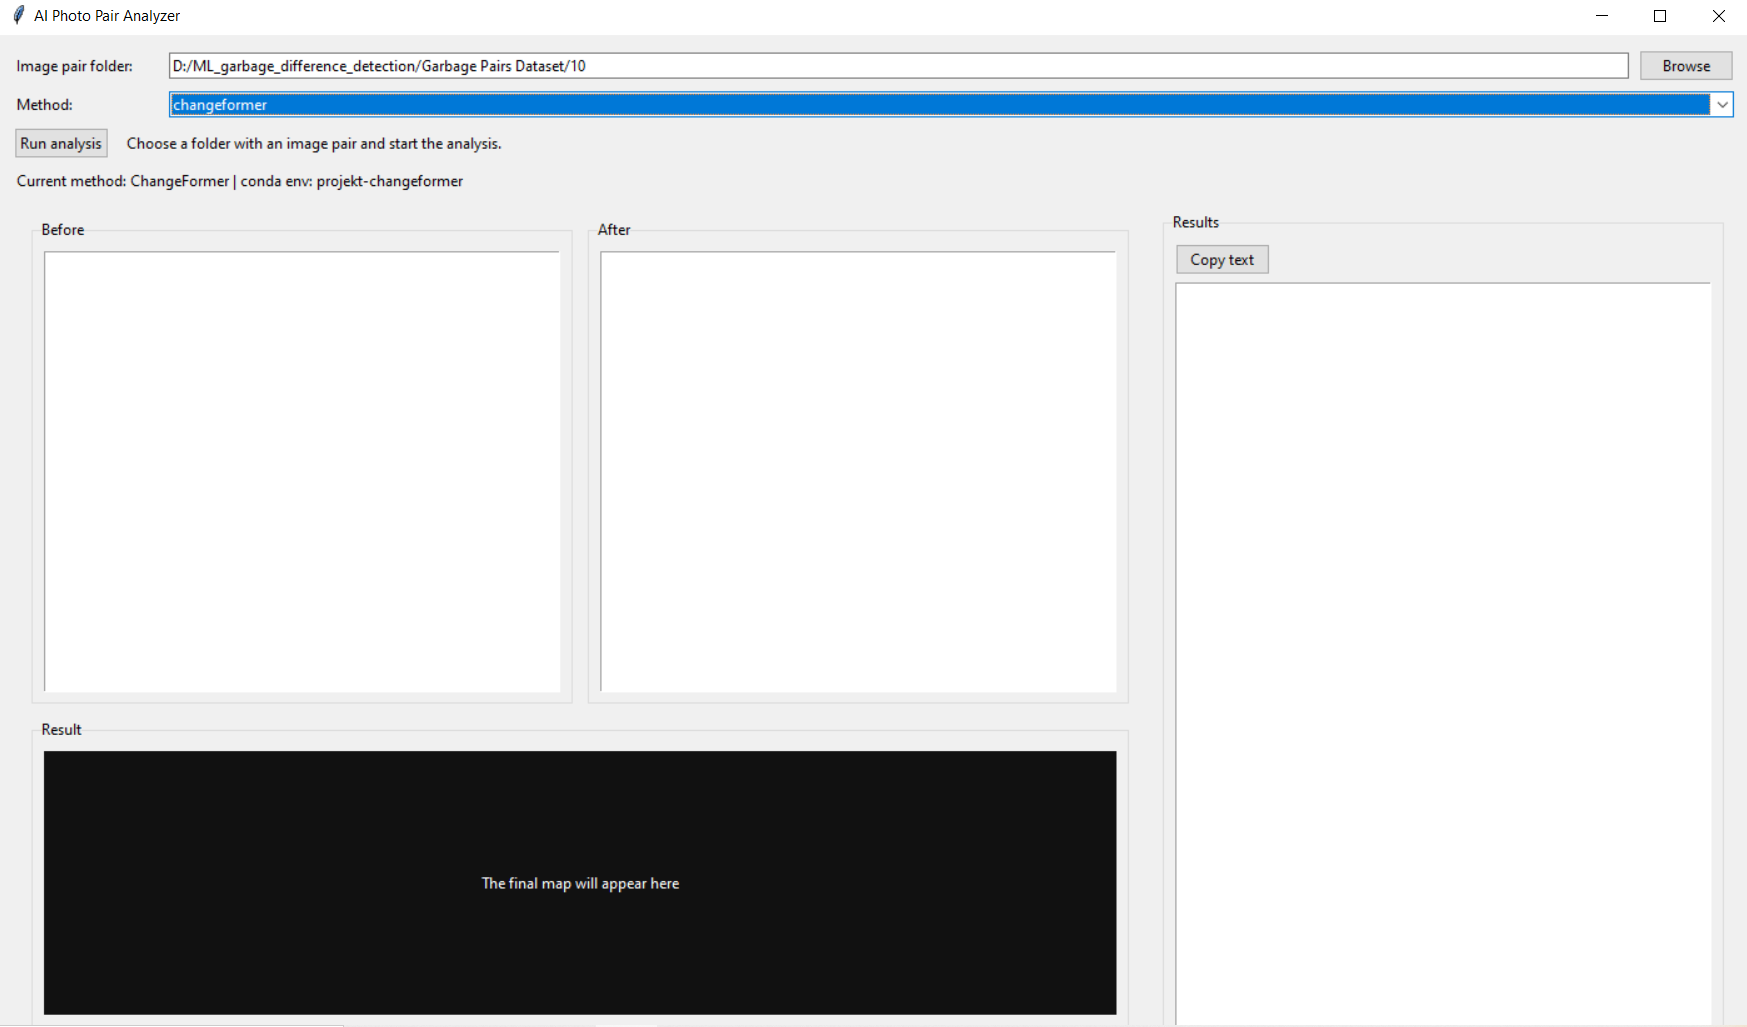
\includegraphics[width=\columnwidth]{foto/interface.png}}
\caption{Používateľské rozhranie programu na analýzu párov fotografií.}
\label{fig:interface}
\end{figure}

\section{YOLOv8-seg}
Metóda YOLOv8-seg slúži na segmentáciu odpadu v jednotlivých snímkach. V našej implementácii sa používa ako samostatná vetva spracovania, ktorá načíta model, vykoná inferenciu nad dvojicou fotografií pred a po vyčistení a následne vytvorí prehľadnú vizualizáciu výsledkov. Metóda pracuje s maskami objektov, takže je vhodná tam, kde chceme presnejšie určiť tvar a rozsah odpadu v scéne \cite{ultralyticsyolo}.

Pri tréningu YOLOv8-seg sme najprv automaticky pripravili export dát z TACO do formátu kompatibilného s Ultralytics. Dataset sa delil na tréningovú, validačnú a testovaciu časť podľa pomeru 80/10/10 a pracoval s jednou triedou ``trash''. Tréning prebiehal približne 90 epoch s malou batch size 2, vstupným rozlíšením 768 px, cache režimom na disku, zapnutým AMP a early stoppingom s patience 20. Ako vstupný checkpoint sa používal predtrénovaný model YOLOv8m alebo záložný YOLOv8s-seg.

Po spracovaní program vytvorí výslednú masku, overlay snímku a textový súhrn s informáciami o priebehu inferencie. Obrázok \ref{fig:yolo} ukazuje príklad výstupu tejto metódy v našej aplikácii.

\begin{figure}[htbp]
\centerline{\includegraphics[width=0.65\columnwidth]{foto/yolo.png}}
\caption{Ukážka výstupu metódy YOLOv8-seg.}
\label{fig:yolo}
\end{figure}

\section{Siamese U-Net}
Siamese U-Net je metóda určená na porovnávanie dvojice snímok pred a po vyčistení. Obe fotografie sa spracúvajú súčasne cez dve vetvy siete, ktoré zdieľajú váhy a vyhodnocujú rozdiely medzi vstupmi. Pred inferenciou sa dvojica zarovná, aby sa znížil vplyv posunu kamery a rozdielneho uhla snímania.

Pri tréningu Siamese U-Net sme používali dve vetvy s encoderom ResNet34 s ImageNet predtrénovaním a decoder pre výstup binárnej change masky \cite{daudt2018fully}. Vstup mal veľkosť 384\,\,x\,\,384 a model sa učil na pároch snímok pred a po spolu s maskami zmeny. Ako loss sme používali kombináciu BCEWithLogitsLoss s váhou pre pozitívne pixely a Soft Dice loss, optimalizácia prebiehala cez AdamW a rozvrh učenia používal CosineAnnealingLR s warmupom. Tréning bol nastavený na 70 epoch, batch size 2, gradient accumulation 4 a early stopping s patience 12.

Výstupom metódy je mapa zmeny a binárna maska oblastí, kde sa pravdepodobne nachádzal odstránený odpad. Následne sa použije jednoduché postprocesovanie, aby sa odstránil šum a zvýraznili súvislé oblasti zmeny. Obrázok \ref{fig:siamese} ukazuje príklad výsledku tejto metódy v programe.

\begin{figure}[htbp]
\centerline{\includegraphics[width=0.65\columnwidth]{foto/siamese.png}}
\caption{Ukážka výstupu metódy Siamese U-Net.}
\label{fig:siamese}
\end{figure}

\section{DINOv2}
DINOv2 v našej implementácii používame ako reprezentáciu obrazu, nie ako samostatne trénovaný segmentačný model \cite{oquab2023dinov2}. Program načíta predtrénovaný backbone z DINOv2 kandidátov \textit{vit\_base\_patch14\_dinov2}, \textit{dinov2\_vitb14} alebo \textit{dinov2\_vits14} cez \textit{timm} alebo \textit{torch.hub}. Ak sa nepodarí použiť transformerový model, metóda sa v tomto kroku neprepína na vlastný tréningový fallback, ale zostane závislá od dostupnosti týchto knižníc.

Pred inferenciou sa dvojica snímok najprv zarovná. Primárne sa skúša ECC affine zarovnanie, a ak to nestačí, použije sa feature-based homography fallback cez SIFT alebo ORB s RANSAC. Až potom sa z oboch obrázkov extrahujú feature gridy z backbone a medzi nimi sa vypočíta cosine distance mapa. Táto mapa sa znormalizuje cez robustné percentily, vyhladí sa a po postprocese sa z nej vytvorí semantická mapa zmien.

Z výstupu sa potom počíta aj odhad miery vyčistenia. Metóda využíva kvalitu zarovnania, lokalizovanú mieru zmeny a textúrovú energiu v zmenených oblastiach. Výsledok sa premietne do hodnoty \textit{cleanup percent} v rozsahu 0 až 100, spolu s príznakom spoľahlivosti a odporúčaním na ručnú kontrolu pri nízkej spoľahlivosti. Obrázok \ref{fig:dino} ukazuje príklad výstupu tejto metódy.

\begin{figure}[htbp]
\centerline{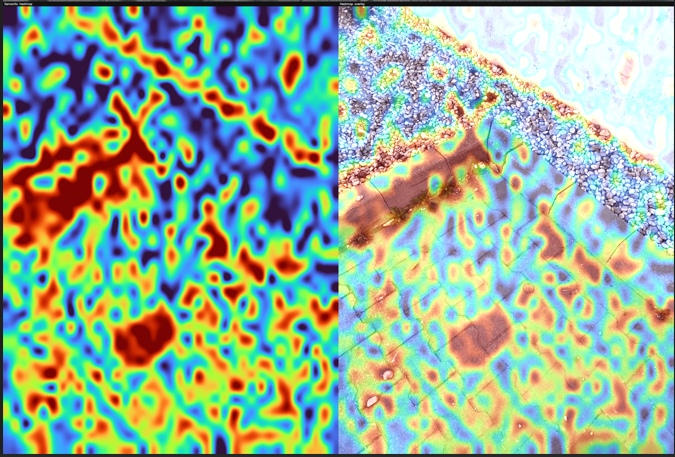
\includegraphics[width=0.85\columnwidth]{foto/dino.png}}
\caption{Ukážka výstupu metódy DINOv2.}
\label{fig:dino}
\end{figure}

\section{ChangeFormer}
ChangeFormer je metóda založená na porovnaní dvojice snímok pomocou transformerových príznakov. V našej implementácii najprv spracuje obrázky po zarovnaní a potom vytvorí mapu zmien v prekrytej oblasti. Ak nie sú dostupné potrebné knižnice alebo model, program automaticky použije klasický CV fallback, aby analýza mohla pokračovať.

Pri tréningu ChangeFormer sme používali dvojice pred a po spolu s binárnymi maskami odstráneného odpadu z vlastného datasetu \cite{changeformer2021}. Dáta sa delili na tréningovú a validačnú časť, vstupy sa menili na fixnú veľkosť a počas učenia sa používali aj augmentácie, aby model lepšie zvládal zmeny uhla záberu a osvetlenia. Optimalizácia prebiehala cez AdamW a loss funkcia kombinovala BCEWithLogitsLoss s Dice loss.

Výsledkom je mapa zmeny, preview obrázok a súbor metrík, medzi ktoré patrí napríklad pomer zmien, kvalita zarovnania a informácia o použitom režime inferencie. Obrázok \ref{fig:changeformer} ukazuje ukážku výstupu tejto metódy.

\begin{figure}[htbp]
\centerline{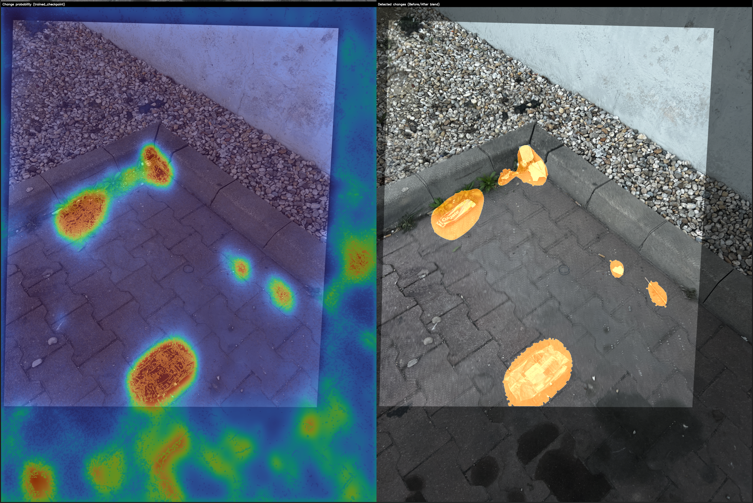
\includegraphics[width=0.85\columnwidth]{foto/ChangeFormer.png}}
\caption{Ukážka výstupu metódy ChangeFormer.}
\label{fig:changeformer}
\end{figure}

\section{EfficientNet}
EfficientNet používame ako pomocný klasifikačný model pre odhad čistého a znečisteného stavu \cite{tan2019efficientnet}. Model dostane dvojicu záberov, vyhodnotí pravdepodobnosť triedy ``dirty'' pre prednú aj zadnú snímku a z týchto hodnôt vypočíta skóre vyčistenia. Ak nie je dostupný natrénovaný checkpoint, runner použije náhradný spôsob odhadu.

Pri tréningu EfficientNet sme binárny dataset tried clean a dirty zostavili z našich pripravených párov pred a po vyčistení a doplnili ho o cropy z TACO. Každý obrázok sa pri tréningu aj inferencii mení na viacero výrezov, aby model nehodnotil iba jeden bod v snímke, ale aj lokálne oblasti so zvyšným odpadom. Z jednotlivých cropov sa potom vypočíta pravdepodobnosť triedy dirty a finálna hodnota sa zloží ako vážená kombinácia priemeru a maxima cropov:
$$
p_{dirty} = \mathrm{clip}(\alpha \cdot \max(p_i) + (1 - \alpha) \cdot \mathrm{mean}(p_i), 0, 1),
$$
pričom $p_i$ sú dirty pravdepodobnosti jednotlivých cropov a $\alpha$ je váha nastavená v konfigurácii. Z tejto hodnoty sa dopočíta $p_{clean} = 1 - p_{dirty}$ a výsledná label sa určuje podľa prahu pre dirty triedu. Skóre vyčistenia sa potom počíta ako
$$
\mathrm{cleanup\_score} = \mathrm{clip}(p_{dirty}^{before} - p_{dirty}^{after}, 0, 1),
$$
čiže vyjadruje, o koľko klesla pravdepodobnosť znečistenia po vyčistení. V tréningu sa používali výrazné obrazové augmentácie, CrossEntropyLoss s váhami tried, optimalizátor AdamW a rozvrh učenia CosineAnnealingLR.

Táto metóda je vhodná na rýchle porovnanie dvoch stavov miesta a na získanie jednoduchého číselného skóre, ktoré dopĺňa segmentačné a change-detection výstupy. Obrázok \ref{fig:efficientnet} zobrazuje príklad výsledku v aplikácii.

\begin{figure}[htbp]
\centerline{\includegraphics[width=0.85\columnwidth]{foto/efficientNet.png}}
\caption{Ukážka výstupu metódy EfficientNet.}
\label{fig:efficientnet}
\end{figure}

\section{SIFT + RANSAC}
Klasická metóda SIFT + RANSAC slúži na zarovnanie dvoch fotografií pomocou bodových príznakov \cite{lowe2004distinctive,fischler1981random}. Najprv sa nájdu zodpovedajúce kľúčové body, následne sa pomocou RANSAC odfiltrujú chybné zhody a fotografie sa premietnu na spoločné plátno. Až potom sa vypočíta diferenčná mapa iba v oblasti prekrytia.

Táto vetva je užitočná najmä v situáciách, kde chceme mať jednoduchý a interpretovateľný základ porovnania bez nutnosti hlbokého modelu. Výstup obsahuje zarovnanie, počet zhôd a inlierov, ako aj mapu zmien v prekrytej oblasti. Obrázok \ref{fig:sift_ransac} ukazuje ukážku výsledku tejto metódy.

\begin{figure}[htbp]
\centerline{
\includegraphics[width=0.85\columnwidth]{\detokenize{foto/sift ransac.png}}}
\caption{Ukážka výstupu metódy SIFT + RANSAC.}
\label{fig:sift_ransac}
\end{figure}

\section{Kvantitatívne vyhodnotenie}
Tabuľka \ref{tab:mask_metrics} sumarizuje priemerné výsledky na 13 pároch s maskami. Pri metódach, ktoré v tomto exporte nevytvárajú priamo maskové metriky, je uvedený znak ``—''. Z pohľadu priestorového prekrytia vychádza najlepšie samotný ChangeFormer. Siamese U-Net a SIFT + RANSAC dávajú použiteľné, ale slabšie výsledky než ChangeFormer, pričom YOLOv8-seg poskytuje hlavne dobrý odhad množstva, no v tomto reporte preň nie sú dostupné Dice a IoU.

\begin{table*}[!t]
\centering
\caption{Priemerné metriky na 13 pároch s maskami. Znak ``—'' znamená, že daná metrika nebola pre metódu v tomto exporte dostupná.}
\label{tab:mask_metrics}
\resizebox{\textwidth}{!}{%
\begin{tabular}{lccccp{5.2cm}}
\hline
Metóda & Dice $\uparrow$ & IoU $\uparrow$ & MAE $\downarrow$ [px] & MAPE $\downarrow$ [\%] & Poznámka \\
\hline
ChangeFormer & \textbf{0.199} & \textbf{0.128} & 87976.273 & 110.445 & najlepšie prekrytie masky \\
DINOv2 & — & — & — & — & bez maskových metrík v tomto exporte \\
EfficientNet & — & — & — & — & bez maskových metrík v tomto exporte \\
Siamese U-Net & 0.191 & 0.117 & 256632.000 & 717.415 & maskový baseline, silné nadhodnotenie \\
YOLOv8-seg & — & — & 34602.769 & 59.022 & množstvo odhaduje dobre, Dice/IoU nie sú dostupné \\
SIFT + RANSAC & 0.135 & 0.082 & 251414.385 & 342.194 & klasický interpretovateľný baseline \\
\hline
\end{tabular}%
}
\end{table*}

\section{Diskusia}
Výsledky ukazujú, že jednotlivé metódy riešia úlohu z rôznych uhlov pohľadu, preto ich nemožno čítať iba cez jednu metriku. ChangeFormer dosahuje najlepšie priestorové prekrytie masky, a preto je v našej práci najsilnejším kandidátom tam, kde je dôležité presne lokalizovať oblasť zmeny. Siamese U-Net a SIFT + RANSAC fungujú ako použiteľné referenčné prístupy, ale ich priemerné prekrytie je nižšie a výsledky sú viac závislé od kvality zarovnania.

YOLOv8-seg sa v tomto projekte javí ako praktická metóda pre odhad množstva odpadu a pre rýchlu vizuálnu kontrolu, no v aktuálnom exporte pre ňu nemáme priamo dostupné maskové metriky Dice a IoU. DINOv2 a EfficientNet zase nepatria medzi čisté segmentačné prístupy, preto sú vhodné skôr ako doplnkové signály pre posúdenie stavu scény než ako priama náhrada za change detection. Z pohľadu celého riešenia je preto najdôležitejšie, že máme viacero metód s odlišným typom výstupu: presnú masku zmeny, odhad množstva a klasifikačné skóre čistoty.

Doplnkový výsledok sme získali aj pri testovaní modelu ChatGPT 5.5 na pároch fotografií. Model veľmi dobre identifikoval prítomnosť odpadu, najmä drobné objekty ako ohorky cigariet, a vedel pomerne presne opísať aj relatívnu polohu zvyšného odpadu v scéne. Na druhej strane, pri priamom vyznačovaní odpadu do obrázka bol výsledok výrazne slabší a masky boli nepresné, takže tento typ výstupu je pre neho stále problematický.

\section{Obmedzenia}
Najväčším obmedzením hodnotenia je malý počet párov, pre ktoré máme vytvorené masky. Na úplne férové porovnanie segmentačných metód by bolo potrebné viac ručne označených dát a rovnomernejšie zastúpenie rôznych typov scén.

Treba tiež zdôrazniť, že všetky metódy neprodukujú rovnaký typ výstupu. Segmentačné a change-detection modely sa prirodzene hodnotia cez Dice, IoU alebo podobné maskové metriky, zatiaľ čo klasifikačné a odhadové metódy skôr cez chybu množstva alebo skóre čistoty. Preto tabuľka slúži hlavne ako praktické porovnanie správania metód, nie ako úplne jednotný benchmark. 

Ďalším zdrojom neistoty je citlivosť na zarovnanie dvojice fotografií. Pri silnejšom posune kamery, inom uhle snímania alebo výrazných zmenách osvetlenia môžu niektoré metódy reagovať na nežiaduce vizuálne rozdiely namiesto skutočného odpadu. Z tohto dôvodu je celé riešenie najspoľahlivejšie ako porovnávacia a diagnostická platforma, nie ako finálny univerzálny rozhodovací systém.

\section{Záver}
V práci sme navrhli a implementovali systém na analýzu dvojíc fotografií pred a po čistiacej akcii, ktorý spája zarovnanie snímok, viacero metód detekcie zmien a grafické používateľské rozhranie. Vytvorili sme aj vlastnú dátovú sadu párov a doplnili ju o ručne pripravené masky pre časť scenárov, aby bolo možné metódy porovnávať na spoločnom základe.

Na základe realizovaných experimentov sa ukázalo, že najlepšie maskové prekrytie dosahuje ChangeFormer, zatiaľ čo YOLOv8-seg a EfficientNet sú užitočné skôr ako doplnkové vetvy pre odhad množstva odpadu a čistoty scény. SIFT + RANSAC a Siamese U-Net poskytujú zrozumiteľné referenčné výsledky, ale ich kvalita závisí najmä od zarovnania a od charakteru scény. DINOv2 sa v riešení uplatnil ako silný reprezentančný základ a ako zdroj doplnkového signálu pre robustnejšie hodnotenie.

Celkový prínos práce spočíva v tom, že vznikla porovnávacia platforma, ktorá umožňuje analyzovať rovnakú dvojicu snímok viacerými prístupmi a interpretovať výsledok z pohľadu segmentácie, odhadu množstva aj klasifikácie. Ďalší vývoj by mal smerovať najmä k rozšíreniu ručne anotovaných dát, zlepšeniu vyhodnotenia na väčšom počte scén a k presnejšiemu kalibrovaniu metrík pre jednotlivé typy modelov.

\begin{thebibliography}{00}
\bibitem{lowe2004distinctive}
D. G. Lowe, ``Distinctive image features from scale-invariant keypoints,'' \emph{International Journal of Computer Vision}, vol. 60, no. 2, pp. 91--110, 2004.

\bibitem{fischler1981random}
M. A. Fischler and R. C. Bolles, ``Random sample consensus: A paradigm for model fitting with applications to image analysis and automated cartography,'' \emph{Communications of the ACM}, vol. 24, no. 6, pp. 381--395, 1981.

\bibitem{daudt2018fully}
J. Daudt, B. Le Saux, and A. Boulch, ``Fully convolutional siamese networks for change detection,'' in \emph{Proc. IEEE Int. Conf. Image Processing (ICIP)}, 2018, pp. 4063--4067.

\bibitem{tan2019efficientnet}
M. Tan and Q. V. Le, ``EfficientNet: Rethinking model scaling for convolutional neural networks,'' in \emph{Proc. Int. Conf. Machine Learning (ICML)}, 2019, pp. 6105--6114.

\bibitem{changeformer2021}
H. Chen and Z. Shi, ``ChangeFormer: A transformer-based siamese network for change detection,'' arXiv:2108.12311, 2021.

\bibitem{oquab2023dinov2}
M. Oquab \emph{et al.}, ``DINOv2: Learning robust visual features without supervision,'' arXiv:2304.07193, 2023.

\bibitem{ultralyticsyolo}
Ultralytics, ``Ultralytics YOLO Documentation,'' 2026. [Online]. Available: https://docs.ultralytics.com/. Accessed: May 13, 2026.
\end{thebibliography}

\end{document}
